\section{Concurrency Control}
\url{../other/professor's slides/2-ConcurrencyControl.pdf}\newline
\newline
The \textbf{concurrency control system}:
\begin{itemize}
    \item manage the simultaneous execution of transactions;
    \item avoids the insurgence of anomalies;
    \item ensure performance: exploit parallelism to maximise transactions per
    second.
\end{itemize}
\ \newline
Two transaction can have a \textbf{serial} execution, an \textbf{interleaved} execution or a \textbf{neasted} execution.
\begin{center}
    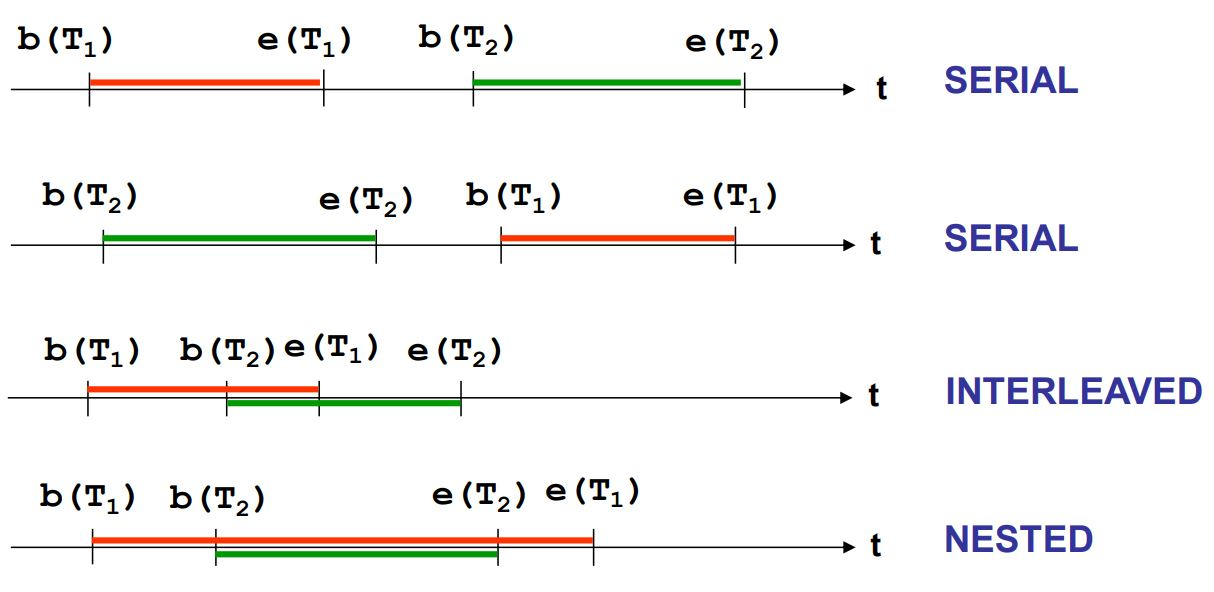
\includegraphics[height=4cm]{../arguments/serial-interleaved-nested.JPG}
\end{center}
\subsection{Anomalies}
An anomalie happens when two transaction are executed interleaved or nested and the result is different if they were executed serially.
\subsubsection{Lost Update}
\[
    r_1(x) \; \rightarrow \; r_2(x) \; \rightarrow \; w_1(x) \; \rightarrow \; w_2(x)
\]
An update is applied from a state that ignores a preceding update, wich is lost.
\subsubsection{Dirty Read}
\[
    r_1(x) \; \rightarrow \; w_1(x) \; \rightarrow \; r_2(x) \; \rightarrow \; abort_1 \; \rightarrow \; w_(2)
\]
An uncommitted value is used to update the data.
\subsubsection{Nonrepeatable Read}
\[
    r_1(x) \; \rightarrow \; r_2(x) \; \rightarrow \; w_2(x) \; \rightarrow \; r_1(x)
\]
Someone else updates a previously read value.
\subsubsection{Phantom Update}
\[
    r_1(x) \; \rightarrow \; r_2(x) \; \rightarrow \; w_2(x) \; \rightarrow \; r_1(x)
\]
Someone else updates data that contributes to a previously read datum.\newline
\newline
Lets see an example: given the costraint $A+B+C = 100$ and the initial values $A = 50, B = 30, C = 20$\newline
$T_1 : r(A), r(B)$\newline
$T_2 : r(B), r(C)$\newline
$T_2 : $ subtract $10$ from $C$ and add $10$ to $B$.\newline
$T_2 : w(B), w(C)$\newline
$T_1 : r(C)$ ($T_1$ reads that the sum is $90$).\newline
So for $T_1$ it is as if "somebody else" had updated the value o the sum, but for $T_2$ the update is perfectly legal (does not change the value of the sum). 
\subsubsection{Phantom Insert}
\[
    r_1(x) \; \rightarrow \; w_2(new\; tuple) \; \rightarrow \; r_1(x)
\]
Someone else inserts dataa that contributes to a previously read datum.\newline
\newline
This anomaly does not depend on data already present in the DB when $T_1$ executes, but on a “phantom” tuple that is inserted by “someone else” and satisfies the conditions of a previous query of $T_1$.
\subsection{Principles of Concurrency Control}
\textbf{Operations}: a read or write of a specific datum by a specific transaction.\newline
\newline
\textbf{Schedule}: a sequence of operations performed by concurrent transactions that respects the order of operations of each transaction.\newline
How many distinct schedules exist for $n$ transaction each with $k_i$ operations?
\[
    N_D = \frac{\left(\sum_{i=1}^{n}k_i\right)!}{\Pi_{i=1}^n (k_i !)}
\]
How many of them are serial?
\[
    N_S = n!
\]
\ \newline
\textbf{Scheduler}: a component that accepts or rejects the operations requested by the transactions.\newline
\newline
\textbf{Serial schedule}: a schedule in which the actions of each transaction occur in a contiguos sequence.
\subsubsection{Serializable schedule}
A \textbf{serializable schedule} is a schedule that leaves the database in the \textbf{same state} as \textbf{some} serial schedule of the same transactions.
\begin{center}
    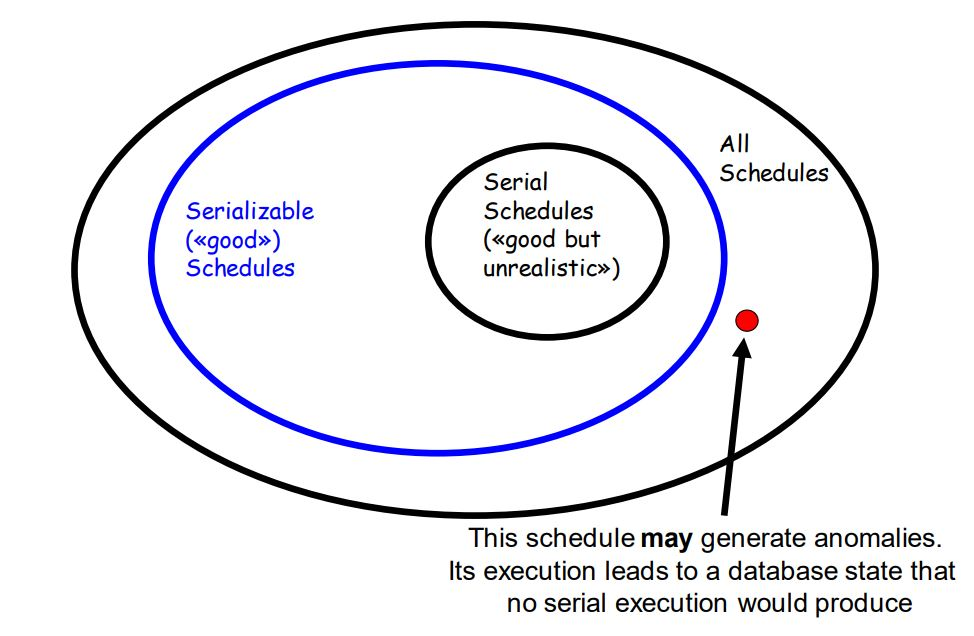
\includegraphics[height=6cm]{../arguments/serializableSchedules.JPG}
\end{center}
\subsubsection{View-serializability}
$r_i(x)$ \textbf{reads-from} $w_j(x)$ in a schedule $S$ when $w_j(x)$ precedes $r_i(x)$ and there is no $w_k(x)$ in $S$ between $r_i(x)$ and $w_j(x)$.\newline
\newline
$w_i(x)$ in a schedule $S$ is a \textbf{final write} if it is the last write on $x$ that occurs in $S$.\newline
\newline
Two schedules are \textbf{view-equivalent} if they have the same operations, the same reads-from relation, and the same final writes.\newline
\newline
A schedule is \textbf{view-serializable} if it is view-equivalent to a serial schedule of the same transactions.\newline
The class of view-serializable schedules is named \textbf{VSR}.\newline
$S$ is \textbf{view-serializable} if:
\begin{enumerate}
    \item every read operation sees the same values;
    \item the final value of each object is written by the same transaction as if the transactions were executed serially in some order.
\end{enumerate}
\ \newline
Deciding if a generic schedule is in VSR is an \textbf{NP-complete problem} but is an heavy task, so we look for a stricter definition that is easier to check, even if we reject sosme schedule that would be acceptable: VSR schedules are "too many".
\subsubsection{Conflict-serializability}
Two operations $o_i$ and $o_j$ are in \textbf{conflict} if they address the same resource and at least one of them is a write: \textbf{read-write} conflicts (r-w or w-r) and \textbf{write-write} conflicts (w-w).\newline
\newline
Two schedules are \textbf{conflict-equivalent} if contain the same operations and in all conflicting pairs transactions occur in the same order.\newline
\newline
A schedule is \textbf{conflict-serializable} if it is conflict-equivalent to a serial schedule of the same transactions.\newline
The class of conflict-serializable schedules is named \textbf{CSR}.
\newline
\newline
All conflict-serializable schedules are also view-serializable, but the inverse is not necessarily true: $CSR \rightarrow VSR$.
\begin{center}
    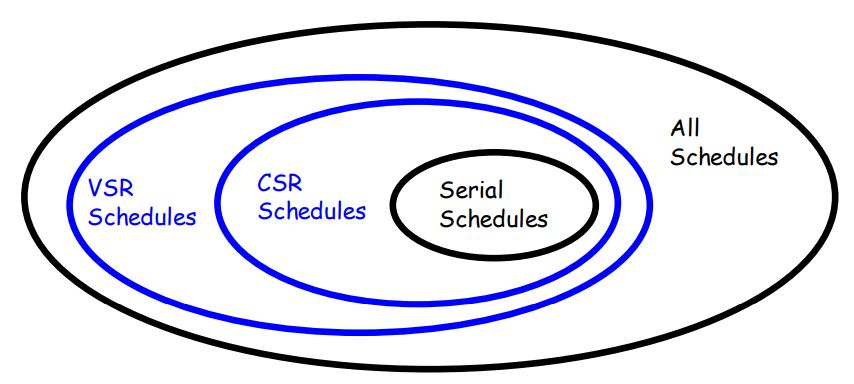
\includegraphics[height=5cm]{../arguments/CSRandVSR.JPG}
\end{center}
\subsubsection{Testing conflict-serializability}
To check if a schedule is conflict-serializable we use a \textbf{conflict graph}:
\begin{itemize}
    \item one node for each transaction $T_i$;
    \item one arc from $T_i$ to $T_j$ if there exists at least one conflict between an operation $o_i$ of $T_i$ and an operations $o_j$ of $T_j$ such that $o_i$ precedes $o_j$;
    \item a schedule is in CSR if and only if its conflict graph is \textbf{acyclic}.
\end{itemize}
To check if a graph is acyclic we use this algorithm:
\begin{itemize}
    \item if a graph is acyclic, then it must have at least one node with no targets, called leaf (with no arrows going away from the node).
    \item if we "peel off" a leaf in an acyclic graph, then we are always left with an acyclic graph, and if we keep peeling off leaf nodes, one of two things will happen: we will eventually peel off al node and so the graph is acyclic, or we will get to a point where there is no leaf, yet the graph is not empty and so the graph is cyclic.
\end{itemize}
If $S$’s graph is acyclic then it induces a \textbf{topological (partial) ordering} on its nodes, that is easier to understand graphically with an example:
\begin{center}
    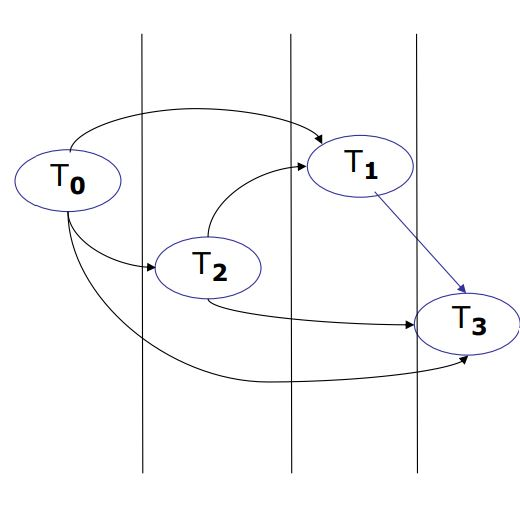
\includegraphics[height=5cm]{../arguments/topologicalpartialorderingCSR.JPG}
\end{center}
In general, there can be many compatible serial schedules.
\subsection{Concurrency control approaches: locking}
Everything we have seen untill now is based on study of schedules after they have been executed. In real life we need a system that can assure cocnurrency control in "live".\newline
There are two main families of techniques:
\begin{itemize}
    \item Pessimistic: based on locks, resource access control.
    \item Optimistic: based on timestamps and versions, serve as many requests as possible, possibly using out-of-date versions of the data.
\end{itemize}
\subsubsection{Locking}
A transaction is \textbf{well-formed w.r.t. locking} if
\begin{itemize}
    \item read operations are preceded by \textbf{r\_lock} (shared lock) and followed by \textbf{unlock};
    \item write operations are preceded by \textbf{w\_lock} (exclusice lock) and followed by \textbf{unlock}.
\end{itemize}
\ \newline
Transactions that first read and then write an object may:
\begin{itemize}
    \item acquire a w\_lock already when reading or
    \item acquire a r\_lock first and then upgrade it into a w\_lock (lock escalation).
\end{itemize}
\ \newline
Possible states of an object:
\begin{itemize}
    \item free;
    \item r-locked (locked by one or more readers);
    \item w-locked (locked by a writer);
\end{itemize}
\ \newline
When a lock request is granted, the resource is acquired; when an unlock is executed, the resource becomes available.\newline
The lock manager grants access to resources according to the \textbf{conflict table}:
\renewcommand{\arraystretch}{1.5}
\begin{center}
    \begin{tabular}{ |c|c c c| } 
     \hline
     & FREE & R\_LOCKED & W\_LOCKED \\ 
     \hline
     r\_lock & OK (R\_LOCKED) & OK (R\_LOCKED n++) & NO (W\_LOCKED) \\ 
     w\_lock & OK (W\_LOCKED) & NO (R\_LOCKED) & NO (W\_LOCKED)\\ 
     unlock & ERROR & OK (DEPENDS n- -) & OK (FREE) \\ 
     \hline
    \end{tabular}
\end{center}
\renewcommand{\arraystretch}{1}
where $n$ is the counter of the current readers